%%%%%%%%%%%%%%%%%%%%%%%%%%%%%%%%%%%%%%%%%%%%%%%%%%%%%%%%%%%%%%%%%%%%%%%%%%%%%%%%%%%%%%%%%%%%%%%%%%%
\documentclass[10pt, a4paper]{article}
%%%%%%%%%%%%%%%%%%%%%%%%%%%%%%%%%%%%%%%%%%%%%%%%%%%%%%%%%%%%%%%%%%%%%%%%%%%%%%%%%%%%%%%%%%%%%%%%%%%

%--------------------------------------------------------------------------------------------------
% Dimensions :
%--------------------------------------------------------------------------------------------------

\setlength{\textheight}{25cm}
\setlength{\textwidth}{16cm}

\setlength{\topmargin}{-20mm}
\setlength{\oddsidemargin}{0mm}
\setlength{\evensidemargin}{0mm}

% \setlength{\columnsep}{20mm}

\setlength{\fboxsep}{1mm}
\setlength{\unitlength}{1mm}

%--------------------------------------------------------------------------------------------------
% Packages :
%--------------------------------------------------------------------------------------------------

\usepackage{latexsym}
\usepackage{graphicx}
\usepackage{pifont}
\usepackage{color}
\usepackage{amsmath}
\usepackage{amssymb}
\usepackage{yhmath}
\usepackage[french]{babel}    % pour franciser le document

%\usepackage[latin1]{inputenc} % pour utiliser les caracteres accentues du claviers
\usepackage[utf8]{inputenc} 

%--------------------------------------------------------------------------------------------------
% Divers :
%--------------------------------------------------------------------------------------------------

\definecolor{bleu}{rgb}{0.2, 0.5, 0.7}

\usepackage{accents}


% Style des vecteurs : fleche ou gras ?

%\newcommand{\myvec}[1]{\boldsymbol{#1}}
\newcommand{\myvec}[1]{\vec{#1}}

\newcommand{\mytensor}[1]{\accentset{\Rightarrow}{#1}} % needs \usepackage{accents}

%---------------------------
% Operateurs differentiels :
%---------------------------

\newcommand{\divergence}{\mbox{\rm div}\,}

\newcommand{\gradient}{\myvec{\mbox{\rm gra}}\mbox{\rm d}}
% \newcommand{\gradient}{\mathbf{grad}\,}
% \newcommand{\ggradient}{\stackrel{\Rightarrow}{\mbox{gra}}\!\!\!\,\mbox{d}\,}
\newcommand{\ggradient}{\accentset{\Rightarrow}{\mbox{\rm gra}}\mbox{\rm d}\!}

%\renewcommand{\dot}[1]{\accentset{\hbox{\huge .}}{#1}}
\newcommand{\mydot}[1]{\accentset{\centerdot}{#1}}

\newcommand{\rot}{\vec{\mbox{\rm ro}}\mbox{\rm t}\,}
%\newcommand{\rot}{\mathbf{rot}\,}

% \newcommand{\vnabla}{\vec{\nabla}}
\newcommand{\vnabla}{\boldsymbol{\nabla}}

% Fonctions speciales:

\newcommand{\besselj}[1]{\mbox{J}_{#1}}
\newcommand{\besselk}[1]{\mbox{K}_{#1}}
\newcommand{\bessely}[1]{\mbox{Y}_{#1}}
\newcommand{\besseli}[1]{\mbox{I}_{#1}}

% Vecteurs, tenseurs et torseurs:

\newcommand{\ex}{\myvec{e}_{x}}
\newcommand{\ey}{\myvec{e}_{y}}
\newcommand{\ez}{\myvec{e}_{z}}

\newcommand{\er}{\myvec{e}_{r}}
\newcommand{\erho}{\myvec{e}_{\rho}}
\newcommand{\ephi}{\myvec{e}_{\varphi}}
\newcommand{\etheta}{\myvec{e}_{\theta}}

%\newcommand{\tensor}[1]{\stackrel{\Rightarrow}{#1}}
\newcommand{\tensor}[1]{\mbox{\sl \textbf{#1}}}
\newcommand{\torseur}[4]{
   \!\!\!\! \left . \begin{array}{c} \\ \\ _#1 \end{array} \!\!\!
   \right \{ \!\!\!
   \begin{array}{#4} #2 \\ \\ #3 \end{array}}

% Integrales multiples:

\newcommand{\odblint}[1]{\int\!\!\!\!\!\int_{#1} \hskip -7mm \bigcirc \;}
\newcommand{\dblint}{\int\!\!\!\!\!\int}
\newcommand{\tplint}{\int\!\!\!\!\!\int\!\!\!\!\!\int}

% Fractions:

\renewcommand{\dfrac}[2]{\displaystyle \frac{#1}{#2}}

% Derivees ordinaires et partielles:

\newcommand{\dpdt}[1]{\dfrac{\partial #1}{\partial t}}
\newcommand{\dpdx}[1]{\dfrac{\partial #1}{\partial x}}
\newcommand{\dpdy}[1]{\dfrac{\partial #1}{\partial y}}
\newcommand{\dpdz}[1]{\dfrac{\partial #1}{\partial z}}

\newcommand{\ddpdt}[1]{\dfrac{\partial^2 #1}{\partial t^2}}
\newcommand{\ddpdx}[1]{\dfrac{\partial^2 #1}{\partial x^2}}
\newcommand{\ddpdy}[1]{\dfrac{\partial^2 #1}{\partial y^2}}
\newcommand{\ddpdz}[1]{\dfrac{\partial^2 #1}{\partial z^2}}

\newcommand{\dpdr}[1]{\dfrac{\partial #1}{\partial r}}
\newcommand{\dpdrho}[1]{\dfrac{\partial #1}{\partial \rho}}
\newcommand{\dpdphi}[1]{\dfrac{\partial #1}{\partial \varphi}}
\newcommand{\dpdtheta}[1]{\dfrac{\partial #1}{\partial \theta}}

\newcommand{\ddpdr}[1]{\dfrac{\partial^2 #1}{\partial r^2}}
\newcommand{\ddpdrho}[1]{\dfrac{\partial^2 #1}{\partial \rho^2}}
\newcommand{\ddpdphi}[1]{\dfrac{\partial^2 #1}{\partial \varphi^2}}
\newcommand{\ddpdtheta}[1]{\dfrac{\partial ^2#1}{\partial \theta^2}}

\newcommand{\ddt}[1]{\dfrac{d #1}{dt}}
\newcommand{\ddx}[1]{\dfrac{d #1}{dx}}
\newcommand{\ddy}[1]{\dfrac{d #1}{dy}}
\newcommand{\ddz}[1]{\dfrac{d #1}{dz}}
\newcommand{\ddr}[1]{\dfrac{d #1}{dr}}

\newcommand{\ddtref}[2]{\dfrac{d #1}{dt}_{\! | #2 }}
\newcommand{\dpdtref}[3]{\dfrac{\partial #1}{\partial #2}_{\! | #3 }}

% Misc:

\newcommand{\bareme}[1]{\reversemarginpar \marginpar{%
	\hspace{8mm} \small \makebox[5mm]{/#1}% 
	\begin{picture}(0, 0)\put(0, 0.5){\makebox[12mm]{\dotfill}}\end{picture}%
	}}

\newcommand{\mycaption}[1]{\caption{\sl #1}}

\newcommand{\ligne}[1]{\hrule height #1\linethickness \hfill}

\newcommand{\thickline}[2]{\linethickness{#1} \line(1, 0){#2}}

\newcommand{\myline}{\noindent\underline{\hspace{\textwidth}}}
\newcommand{\mysection}[1]{\vskip 0.5cm \section{#1}\vskip -1.4cm 
   \myline \vskip 0.4cm \myline \bigskip}

\newcommand{\etal}{\textit{et al.}}

\newcommand{\varray}[1]{\renewcommand{\arraystretch}{#1}}

\newcommand{\puissance}[1]{^{\mbox{\footnotesize #1}}}
\newcommand{\indice}[1]{_{\mbox{\footnotesize #1}}}

%---------------------------------------------------------------------
% New environments:
%---------------------------------------------------------------------

\newcounter{MyEnumCounter}
\newcounter{MySaveCounter}
\newenvironment{MyEnum}{%
  \begin{list}{\arabic{MyEnumCounter}.}{\usecounter{MyEnumCounter}%
  \setcounter{MyEnumCounter}{\value{MySaveCounter}}}
  }{%
  \setcounter{MySaveCounter}{\value{MyEnumCounter}}\end{list}%
}
\newcommand{\MyEnumReset}{\setcounter{MySaveCounter}{0}}

\newenvironment{deuxcols}{\begin{tabular}{lr} \hspace*{-9.7mm}}{\end{tabular}}

\newenvironment{dem}{\noindent %
   \begin{tabular}{||l} \textsl{D\'emonstration :} \\ % 
   \begin{minipage}{15.5cm} \footnotesize} %
   {\end{minipage}\end{tabular}}

\newenvironment{abst}{\begin{quotation}\sl}{\end{quotation}}

\newenvironment{eqnbox}{\begin{equation}\begin{array}{|c|}  \hline \\ 
   \displaystyle}{\\ \\ \hline \end{array} \end{equation}}

% JFM symbols:

\DeclareMathSymbol{\varGamma}{\mathord}{letters}{"00}
\DeclareMathSymbol{\varDelta}{\mathord}{letters}{"01}
\DeclareMathSymbol{\varTheta}{\mathord}{letters}{"02}
\DeclareMathSymbol{\varLambda}{\mathord}{letters}{"03}
\DeclareMathSymbol{\varXi}{\mathord}{letters}{"04}
\DeclareMathSymbol{\varPi}{\mathord}{letters}{"05}
\DeclareMathSymbol{\varSigma}{\mathord}{letters}{"06}
\DeclareMathSymbol{\varUpsilon}{\mathord}{letters}{"07}
\DeclareMathSymbol{\varPhi}{\mathord}{letters}{"08}
\DeclareMathSymbol{\varPsi}{\mathord}{letters}{"09}
\DeclareMathSymbol{\varOmega}{\mathord}{letters}{"0A}

% ---------------------------------------------------------------------
% MISC SYMBOLS :
% ---------------------------------------------------------------------

\font\SY=msam10 
\def\carreblanc{\hbox{\SY \char'3}}
\def\carrenoir{\hbox{\SY \char'4}}
\def\diamblanc{\hbox{\SY \char'6}}
\def\diamnoir{\hbox{\SY \char'7}}
\def\triblancright{\hbox{\SY \char'102}}
\def\triblancleft{\hbox{\SY \char'103}}
\def\triblancup{\hbox{\SY \char'115}}
\def\triblancdown{\hbox{\SY \char'117}}
\def\trinoirright{\hbox{\SY \char'111}}
\def\trinoirleft{\hbox{\SY \char'112}}
\def\trinoirup{\hbox{\SY \char'116}}
\def\trinoirdown{\hbox{\SY \char'110}}
\def\rondblanc{\hbox{\scriptsize $\bigcirc$}}
\def\rondnoir{\hbox{\LARGE $\bullet$}}

\font\BB=msbm10 scaled 1095
\def\setr{\hbox{\BB R}}
\def\setc{\hbox{\BB C}}
\def\setn{\hbox{\BB N}}
\def\setz{\hbox{\BB Z}}

% Pour enlever la numerotation des pages de la table des matieres:

%%%% debut macro, a placer dans preambule %%%%
\makeatletter
\def\addcontentsline@toc#1#2#3{%
   \addtocontents{#1}{\protect\thispagestyle{empty}}%
   \addtocontents{#1}{\protect\contentsline{#2}{#3}{\thepage}}}
\def\addcontentsline#1#2#3{%
  \expandafter\@ifundefined{addcontentsline@#1}%
  {\addtocontents{#1}{\protect\contentsline{#2}{#3}{\thepage}}}
  {\csname addcontentsline@#1\endcsname{#1}{#2}{#3}}}
\makeatother
%%%% fin macro %%%%

\newcommand{\titre}[1]{ %
  \medskip \noindent \underline{\makebox[\textwidth][l]{\textbf{#1}\textcolor{white}{pl}}}}% \\}

\newcommand{\sstitre}[1]{ %
  \bigskip \centerline{\textbf{#1}} \smallskip}

\def\draft{\overfullrule 5pt} % The \draft command marks the overful boxes

\def\indentlist{\list%
        {}{\labelwidth 0pt \leftmargin 3\labelsep}}
\let\endindentlist\endlist \relax

\def\datelist{\list%
        {}{\settowidth\labelwidth{[2001/02 :]}
        \leftmargin\labelwidth
        \advance\leftmargin\labelsep}
}
\let\enddatelist\endlist \relax

\def\longuelist{\list%
        {}{\settowidth\labelwidth{[Etablissement :]}
        \leftmargin\labelwidth
        \advance\leftmargin\labelsep}
}
\let\endlonguelist\endlist \relax

\def\shortlist{\list%
        {}{\settowidth\labelwidth{$\bullet$}
        \leftmargin\labelwidth
        \advance\leftmargin\labelsep}
}
\let\endshortlist\endlist \relax



\renewcommand{\thickline}[2]{\linethickness{#1} \line(1, 0){#2}}
\renewcommand{\mycaption}[1]{\caption{\sl #1}}
\renewcommand{\myvec}[1]{\vec{#1}}

%\pagestyle{empty}

\graphicspath{{../FIGURES/}{Figures/}} % chemin d'acces au repertoire des figures (par ex.)

%%%%%%%%%%%%%%%%%%%%%%%%%%%%%%%%%%%%%%%%%%%%%%%%%%%%%%%%%%%%%%%%%%%%%%%%%%%%%%%%%%%%%%%%%%%%%%%%%%%
\begin{document}
%%%%%%%%%%%%%%%%%%%%%%%%%%%%%%%%%%%%%%%%%%%%%%%%%%%%%%%%%%%%%%%%%%%%%%%%%%%%%%%%%%%%%%%%%%%%%%%%%%%

\begin{center}

  \textsc{Université Toulouse 3 -- Paul Sabatier \hfill Année universitaire 2017-2018}
  
  \textsc{Mécanique des fluides \hfill L3 Mécanique}
  
  \vspace{0mm}
  
  \begin{center}
    \thickline{0.4mm}{160}
    \\ \vspace{3mm}
  \textbf{\large Exercice complémentaire chapitre Cinématique : écoulements linéaires (correction)}
    \\ %\vspace{1mm}
    \thickline{0.4mm}{160}
  \end{center}

%  \vspace{0mm}
  
\end{center}

%\stepcounter{section}

\medskip

%==================================================================================================
\section{Introduction}
%==================================================================================================

\begin{enumerate}
\item
$\divergence \myvec{u} 
= \dpdx{u} + \dpdy{v} 
= a + d 
$
%= \dpdx{}\left (\dpdy{\psi}\right) + \dpdy{}\left (-\dpdx{\psi}\right)
%= \dfrac{\partial \psi}{\partial x \partial y} - \dfrac{\partial \psi}{\partial y \partial x}
%= \fbox{$0$}$

\item
%Considérons $\psi_1$ et $\psi_2$ solutions du système (2). On a alors :
%$u = \dpdy{\psi_1} = \dpdy{\psi_2} 
%\Leftrightarrow \dpdy{}\left ( \psi_1-\psi_2 \right) = 0$ 
%
%\medskip
%donc $\psi_1-\psi_2 = f(x)$ où $f$ est une fonction qu'il reste à déterminer.
%
%\medskip
%Si $\psi_1$ et $\psi_2$ sont solutions du système (2), on a aussi :
%$v = -\dpdx{\psi_1} = -\dpdx{\psi_2} 
%\Leftrightarrow \dpdx{}\left ( \psi_1-\psi_2 \right) = 0$.
%
%\medskip
%Comme $\psi_1-\psi_2 = f(x)$, on en déduit $f'(x) = 0$, c'est-à-dire $f(x) = Cte$.
%
%\medskip
%En conclusion si $\psi_1$ et $\psi_2$ sont solutions, alors elles sont identiques à une constante additive près : 
%
%\medskip
%\fbox{$\psi_1(x, y) = \psi_2(x, y) + Cte$}

Si $\divergence \myvec{u} =0$ alors par définition il existe une fonction courant $\psi(x,y)$ vérifiant :
 
 \begin{eqnarray}
\dpdy \psi = u(x,y) &=& a x + by\\
\dpdx \psi = - v(x,y) &=& -cx+ay
\end{eqnarray} 

En intégrant la première équation par rapport à $y$ (à $x$ fixé) on obtient :
$$
\psi(x,y) = b y^2/2 + a xy + F(x)
$$
où $F(x)$ est une "constante d'intégration" (par rapport à $y$) qui est dans le cas général une fonction de $x$.
En dérivant cette deuxième expression et en identifiant avec la relation précédente :
$$
\dpdx \psi = a y + F'(x) = ay -c x
$$
On en déduit $F(x) = -c x^2/2 + cte$. Soit au final :

\fbox{$\psi = - c x^2/2 + b y^2/2 + a xy + C^{te}$}



\medskip
\item
Si $d\myvec{x} = dx\, \ex + dy\,\ey$ désigne un déplacement élémentaire le long d'une ligne de courant,
alors par définition des lignes de courant (qui sont les lignes de champ du champ de vitesse, et 
donc tangentes en tout point à la vitesse locale) :

\medskip
le long de la ligne de courant $d\myvec{x} \wedge \myvec{u} = \myvec{0}
\Leftrightarrow v \, dx - u \, dy = 0
\Leftrightarrow -\dpdx{\psi} \, dx - \dpdy{\psi} \, dy = 0$.

\medskip
Comme la variation élémentaire de $\psi$ s'écrit $d\psi = \dpdx{\psi} \, dx + \dpdy{\psi} \, dy$,
on en déduit que $d\psi=0$ 

\medskip
c'est-à-dire \fbox{$\psi(x, y) = Cte$ le long de la ligne de courant}

\medskip
\item
Considérons une ligne $[A_1A_2]$ 
quelconque reliant deux lignes de courant définies par
$\psi(x, y) = C_1$ et $\psi(x, y) = C_2$ (fig.~\ref{fig:debit}a).

Par définition, le débit à l'instant $t$ passant à travers cette ligne 
est donné par
$q = \displaystyle \int_{A_1}^{A_2} \myvec{u} \cdot \!  \myvec{n} \, dl$

\medskip
où $\myvec{n}$ est la normale locale et où $dl$ désigne le déplacement élémentaire le long de la ligne $[A_1A_2]$. 

\medskip
Le déplacement $dl$ a pour projection $dx$ et $dy$ suivant les directions $x$ et $y$ (fig.~\ref{fig:debit}b), et on en déduit que la normale $\myvec{n}$, vecteur unitaire ($||\myvec{n}|| = 1$) et normal au déplacement élémentaire
($n_x \,dx + n_y \,dy = 0$), s'écrit :

\dotfill
$\myvec{n} = \dfrac{dy}{dl} \, \ex - \dfrac{dx}{dl} \, \ey$, avec
$dl = \sqrt{dx^2 + dy^2}$.

\medskip
On a donc $\myvec{n} \, dl = dy\, \ex - dx\, \ey$, et \dotfill
$\myvec{u} \cdot \! \myvec{n} \, dl 
= u\, dy - v\, dx
= \dpdy{\psi}\, dy + \dpdx{\psi} \, dx = d\psi$

le débit s'écrit alors
$q 
= \displaystyle \int_{A_1}^{A_2} \myvec{u} \cdot \! \myvec{n} \, dl
= \int_{A_1}^{A_2} d\psi
= \psi(A_2) - \psi(A_1)$, 
c'est-à-dire
\fbox{$q = C_2-C_1$}

\begin{figure}[hbt]
\begin{center}
	\begin{picture}(120, 60)(-5, 0)
		\put(0, 0){\includegraphics[width=120mm]{debit.pdf}}
		\put(-20, 46){$\psi(x, y) = C_2$}
		\put(-20, 26){$\psi(x, y) = C_1$}
		\put(14, 35){$dl$}
		\put(32, 28){$\myvec{n}$}
		\put(25, 47){$A_2$}
		\put(12, 20){$A_1$}
		\put(14.5, 23.7){$\bullet$}
		\put(25, 44.5){$\bullet$}
		\put(80, 30){$dl$}
		\put(120, 12){$\myvec{n}$}
		\put(100, 32){$n_x$}
		\put(119, 23){$n_y$}
		\put(83, 16){$d_x$}
		\put(91, 34){$d_y$}
		\put(20, 0){(a)}
		\put(100, 0){(b)}
	\end{picture}
\end{center}
\mycaption{Schéma relatif au calcul du débit entre deux lignes de courant (a).
		Zoom sur le déplacement élémentaire $dl$ (b).}
\label{fig:debit}
\end{figure}

\end{enumerate}

%==================================================================================================
\section{Ecoulements linéaires}
%==================================================================================================

\begin{enumerate}
\item
$u = \dpdy{\psi} = \fbox{$by$}$ et $v = -\dpdx{\psi} = \fbox{$cx$}$

\item
$\divergence \myvec{u} 
= \dpdx{u} + \dpdy{v} 
= \dpdx{}\left ( by \right) + \dpdy{}\left ( -bx \right)
= \fbox{$0$}$

\item
$\myvec{a} = \ddt{\myvec{u}} 
= \dpdt{\myvec{u}} + \left ( \myvec{u} \cdot \gradient \right ) \myvec{u}$

\medskip
c'est-à-dire 
\dotfill $a_x = \dpdt{u} + u \dpdx{u} + v \dpdy{u} = bcx$
et $a_y = \dpdt{v} + u \dpdx{v} + v \dpdy{v} = -bcy$

\medskip
D'où \dotfill 
$\ddt{\myvec{u}} 
= ac x \, \ex+ ac \, \ey 
= ac \left (  x \ex + y\ey \right)$

\medskip
En introduisant les coordonnées polaires, on remarque que
$x \ex + y\ey 
= r\cos \theta \, \ex  + r\sin \theta \, \ey
= r \left (\cos \theta \, \ex  + \sin \theta \, \ey \right )
= r \, \er(\theta)$, où $\er(\theta) = \cos \theta \, \ex  + \sin \theta \, \ey$ est le vecteur radial du repérage polaire (ou cylindrique).

\medskip
En conclusion, la dérivée particulaire est purement radiale :
\dotfill
\fbox{$\ddt{\myvec{u}} = ac \, r\, \er(\theta)$}

\medskip
Dans le cas où les coefficients $a$ et $c$ dépendent du temps, les composantes de la dérivée particulaire s'écrivent alors :

\medskip
$a_x = \dpdt{u} + u \dpdx{u} + v \dpdy{u} = \dot{b}y+acx$
\; et \;  
$a_y = \dpdt{v} + u \dpdx{v} + v \dpdy{v} = \dot{c}x+acy$

où le point désigne la dérivée par rapport au temps.

\medskip
On a donc 
$\ddt{\myvec{u}} 
= \left ( \dot{b}y +ac x \right ) \, \ex 
+ \left ( \dot{c}x  +ac y \right ) \, \ey 
= \fbox{$ac \, r\, \er(\theta) 
+ 2 \left ( \dot{b}y \, \ex + \dot{c}x \, \ey \right )$}$

\item
Le tenseur des gradients des vitesse a pour composantes
$G_{ij} = u_{i, j} = \dfrac{\partial u_i}{\partial x_j}$ (cf. cours de MMC),
avec $u = by$, $v=cx$ et $u_z = 0$ :

\[
	\mytensor{G} =
	\left (
		\begin{array}{ccc}
			\dpdx{u} & \dpdy{u} & \dpdz{u} \\ & & \\
			\dpdx{v} & \dpdy{v} & \dpdz{v} \\ & & \\
			\dpdx{u_z} & \dpdy{u_z} & \dpdz{u_z}
		\end{array}
	\right )
	=
	\left (
		\begin{array}{ccc}
			0 & b & 0 \\ 
			c & 0 & 0 \\
			0 & 0 & 0
		\end{array}
	\right )
\]

Comme $\dpdz{u} = \dpdz{v} = 0$ et $u_z = 0$ dans le cas présent d'un écoulement plan, la dernière colonne et 

\medskip
la dernière ligne du tenseur sont nécessairement nulles. 
On peut donc se restreindre à un tenseur 

\medskip
représenté par la matrice 
$2 \times 2$ constituée des deux premières lignes et colonnes du tenseur complet :

\medskip
\dotfill 
\fbox{$ 	\mytensor{G} = 	\left (
		\begin{array}{cc}
			0 & b \\ 
			c & 0 
		\end{array}
	\right )
$ }

\item
En notant $\myvec{x} = x\ex + y\ey$ le vecteur position, on remarque que
$\myvec{u} = \mytensor{G} \cdot \myvec{x}$.
Le champ de vitesse est donc une fonction linéaire de la position d'où la dénomination d'\,\fbox{écoulement linéaire}

\item
Par définition, le tenseur des taux de déformation est $\mytensor{D} 
= \dfrac{1}{2} \left ( \mytensor{G} + {}^t \mytensor{G} \right )$
où ${}^t$ désigne la transposée :

\medskip
$
	\mytensor{D} = \dfrac{1}{2} \left [
	 \left (
		\begin{array}{cc}
			0 & b \\ 
			c & 0 
		\end{array}
	\right )
+
\left (
		\begin{array}{cc}
			0 & c \\ 
			b & 0 
		\end{array}
	\right )
\right ]
$
\dotfill
\fbox{$ \mytensor{D} = 	 \left (
		\begin{array}{cc}
			0 & (b+c)/2 \\ 
			(b+c)/2 & 0 
		\end{array}
	\right )
$}

\medskip
Le tenseur des taux de déformation est donc nul pour \fbox{$b=-c$}

\item
Par définition, le tenseur des taux de rotation est $\mytensor{R} 
= \dfrac{1}{2} \left ( \mytensor{G} - {}^t \mytensor{G} \right )$
où ${}^t$ désigne la transposée :

\medskip
$
	\mytensor{R} = \dfrac{1}{2} \left [
	 \left (
		\begin{array}{cc}
			0 & b \\ 
			c & 0 
		\end{array}
	\right )
-
\left (
		\begin{array}{cc}
			0 & c \\ 
			b & 0 
		\end{array}
	\right )
\right ]
$
\dotfill

\fbox{ $\mytensor{R} = 	 \left (
		\begin{array}{cc}
			0 & (b-c)/2 \\ 
	(c-b)/2 & 0 
		\end{array}
	\right )
$}

\medskip
Le tenseur des taux de rotation est donc nul pour \fbox{$c=b$}

\item
En s'inspirant de la décomposition canonique du tenseur des gradients de vitesse, on peut essayer d'écrire la fonction de courant en faisant apparaître à part une composante de déformation pure (associée au facteur $c+b$ nul si pas de déformation) et une composante de rotation pure (associée au facteur $c+b$ nul si pas de rotation) :

\dotfill
\fbox{$\psi(x, y) 
= \underbrace{\dfrac{c+b}{2} \left (x^2 + y^2 \right )}_{\mbox{\footnotesize \sl rotation}}
- \underbrace{\dfrac{c-b}{2} \left (x^2 - y^2 \right )}_{\mbox{\footnotesize \sl déformation}}$}

\item
Par définition, le vecteur tourbillon (le vecteur rotation instantané local du fluide) est donné par 

\medskip
$\myvec{\varOmega} 
= \dfrac{1}{2} \, \rot \! \left ( \myvec{u} \, \right )
= \dfrac{1}{2} \, \left (
\begin{array}{c} \dpdx{} \\ \\ \dpdy{} \\ \\ \dpdz{}\end{array} \right )
\wedge
\left (
\begin{array}{c} u \\ \\ \\ v \\ \\ \\ u_z\end{array} \right )
= 
\dfrac{1}{2} \, \left (
\begin{array}{c} 
\dpdy{u_z} - \dpdz{v}
\\ \\
\dpdz{u} - \dpdx{u_z}
\\ \\
\dpdx{v} - \dpdy{u}
\end{array} \right )
= 
\dfrac{1}{2} \, \left (
\begin{array}{c} 
0
\\ \\
0
\\ \\
\dpdx{v} - \dpdy{u}
\end{array} \right )
$

\medskip
car $\dpdz{u} = \dpdz{v} = 0$ et $u_z = 0$ dans le cas présent d'un écoulement plan,

\medskip
d'où
$\myvec{\varOmega} = \dfrac{1}{2}
\left ( \dpdx{v} - \dpdy{u}\right ) \, \ez
$
\dotfill
\fbox{$ \myvec{\varOmega} = (b-c)/2 \, \ez$}

\medskip
On remarque que ce champ est constant en espace : 
il s'agit donc d'un champ \textsl{uniforme}.
Toutes les particules fluides ont la même vitesse angulaire, c'est-à-dire
la même vitesse de rotation sur elles-mêmes.

\medskip
La vorticité est par définition $\myvec{\omega} = 2 \myvec{\varOmega}$
\dotfill
\fbox{$\myvec{\omega} = (b-c)\, \ez)$}

\medskip
On remarque comme précédemment que le champ de vorticité est uniforme.


\item 

On commence par exprimer les anciennes coordonnées $(x,y)$ en fonction des nouvelles :

\medskip 
\dotfill
$x = - x' \cos \theta + y' \sin \theta$ ;  $y = x' \sin \theta + y' \cos \theta$ ;

\medskip 

On utilise cette expression pour exprimer $u$ et $v$ en fonction de $x'$ et $y'$, puis on utilise cette expression pour exprimer $u'$ et $u_ y'$. Ce qui amène à : 

\medskip
\dotfill
$ \left\{ \begin{array}{rcrcl} 
u' &=& (b-c)/2 y' &+& (c+d)/2 \left( 2 \cos \theta \sin \theta x' + [\cos^2 \theta - \sin^2 \theta] y' \right) \\
v' &=& (c-b)/2 x' &+&  (b-x)/2 \left( -2 \cos \theta \sin \theta x' + [\cos^2 \theta - \sin^2 \theta] y' \right) 
\end{array} \right.
$

On en déduit les tenseurs recherchés :


\medskip 
\dotfill
\fbox{ $\mytensor{R}_{(x'y')} = (b+c)/2	 \left(
		\begin{array}{cc}
			0 & 1 \\ 
		-1 & 0 
		\end{array}
	\right) $ }


\medskip 
\dotfill
\fbox{ $ \mytensor{D}_{(x'y')} = (b-c)/2	 \left(
		\begin{array}{cc}
			 2 \cos \theta \sin \theta & \cos^2 \theta - \sin^2 \theta  \\ 
		 \cos^2 \theta - \sin^2 \theta & -2 \cos \theta \sin \theta   
		\end{array}
	\right) $ }


Remarque : on pourrait obtenir directement ces résultats en utilisant la formule de MMC de changement de repère d'un tenseur :


\dotfill 
$\mytensor{G}_{(x'y')} = \mytensor{\Theta}^{-1} \mytensor{G} \mytensor{\Theta}$ 
\quad où $\mytensor{\Theta}$ est la matrice de changement de base :
\quad $
\mytensor{\Theta} = 	 \left(
		\begin{array}{cc}
			 \cos \theta &  \sin \theta  \\ 
		 - \sin \theta & \cos \theta    
		\end{array}
	\right)
$

\medskip

\item On remarque que le tenseur des taux de rotation est invariant par changement de base.



\medskip On remarque que pour la valeur $\theta = \pi/2$ le tenseur devient diagonal :
$ \mytensor{D}_{x'y'} = (b+c)/2 \begin{array}{cc}
			 1 & 0  \\ 
		0 & -1   
		\end{array}
$
Ce choix de base correspond aux {\em axes propres} du tenseur


\end{enumerate}

%==================================================================================================
\section{Tracés graphiques et cas particuliers}
%==================================================================================================

\begin{enumerate}
%\pagebreak

\item

%Le tracé des lignes de courant $\psi(x, y) = Cte$ est accessible
%sous MATLAB avec la commande \texttt{contour}, qui trace les lignes de niveau
%d'un champ scalaire 2D donné.

%Le programme complet est donné sur la page web du cours.


%\medskip
Le programme \texttt{Ecoulements2D.m} est 
disponible sur la page Moodle du cours.%
%\underline{\hspace{150mm}}
%
%\begin{verbatim}
%	clear all; close all; clc;
%	
%	fprintf('\n Trace les lignes de courant pour l''ecoulement defini \n')
%	fprintf(' par la fonction de courant psi(x, y) = -c x^2/2 + b y^2/2 \n\n')
%	
%	% Valeur des paramètres a et b :
%	a = input(' a = ');
%	b = input(' b = ');
%	
%	% Maillage de l'espace avec 100 points entre -1 et 1 en x et y :
%	[x, y] = meshgrid(linspace(-1, 1, 100), linspace(-1, 1, 100));
%	
%	% Definition de la fonction de courant :
%	psi = a*x.^2+b*y.^2;
%	
%	% Trace 10 lignes de courant psi=constante :
%	contour(x, y, psi, 10, 'r');
%	xlabel('x'); ylabel('y');
%	axis equal tight
%	
%	% On peut aussi tracer le champ de vitesse sur un maillage moins fin
%	[x, y] = meshgrid(linspace(-1, 1, 10), linspace(-1, 1, 10));
%	ux =  2*b*y;
%	uy = -2*a*x;
%	hold on
%	quiver(x, y, ux, uy, 'Color', 'b');
%	
%	% On sauvegarde la figure sur le disque :
%	print(gcf, 'streamlines.pdf', '-dpdf');  % format PDF
%	print(gcf, 'streamlines.eps', '-deps');  % format Postscript encapsule
%	print(gcf, 'streamlines.jpg', '-djpeg'); % format JPEG
%\end{verbatim}
%
\underline{\hspace{150mm}}

\bigskip


\item
Cas $c=0$
\medskip
\begin{enumerate}
\item
Lignes de courant $\psi(x, y) = Cte \Leftrightarrow b y^2/2 = Cte \Leftrightarrow y=Cte$ : les lignes de courant sont donc des
\fbox{droites horizontales} (cf. fig.~\ref{fig:streamlines}a).

\medskip
La trajectoire $\myvec{X}(t) = X(t) \, \ex + Y(t) \, \ey$ d'une particule fluide est donnée par
$\dot{\myvec{X}} = \myvec{u}(\myvec{X})$, soit $\dot{X} = b Y$ et $\dot{Y} = 0$.
On en déduit que $Y(t) = Cte = Y_0$, et $X(t) = bY_0\, t + X_0$ : 
les trajectoires sont donc aussi des \fbox{droites horizontales}.

\medskip
\item
L'accélération des particules fluides est donnée par la dérivée particulaire calculée dans 

\medskip
la question 3 
de la section précédente :
$\myvec{a} = acr\, \er = \fbox{$\myvec{0}$}$ dans le cas présent $a=0$.

\medskip
Ce résultat se retrouve en considérant la trajectoire des particules calculées précédemment :

\medskip
$\myvec{X} = \left (bY_0\, t + X_0 \right)\, \ex + Y_0\, \ey$, d'où l'accélération 
$\myvec{a} = \ddot{\myvec{X}} = \myvec{0}$.

\medskip
\item
Dans le cas $c=0$, les tenseurs des taux de déformation et des taux de rotation ont pour 

\medskip
expression :
$\mytensor{D} = 	 \left (
		\begin{array}{cc}
			0 & b \\ 
		b & 0 
		\end{array}
	\right )$
et
$\mytensor{R} = 	 \left (
		\begin{array}{cc}
			0 & b \\ 
		-b & 0 
		\end{array}
	\right ).
$

\medskip
L'écoulement est donc caractérisé par un taux de déformation $b$ qui a la \fbox{même intensité} que 

\medskip
le taux de rotation
(ou vitesse angulaire $\myvec{\varOmega} = -b\, \ez$).

\medskip
Il s'agit d'un écoulement dit de \textsl{cisaillement simple}, aussi appelé parfois \textsl{écoulement de Couette}, dont le profil de vitesse est représentée sur la figure~\ref{fig:couette}.
On obtient ce type d'écoulement par exemple entre deux plaques parallèle en translation horizontale à des vitesses différentes.

\end{enumerate}
\bigskip

\item
Cas $c/b=-1 \Leftrightarrow b=-c$
\medskip
\begin{enumerate}
\item
Lignes de courant $\psi(x, y) = Cte \Leftrightarrow b (x^2/2 + y^2) = Cte \Leftrightarrow x^2+y^2=Cte$ : 

\medskip
les lignes de courant sont donc des
\fbox{cercles concentriques} (cf. fig.~\ref{fig:streamlines}b).

\medskip
La trajectoire $\myvec{X}(t) = X(t) \, \ex + Y(t) \, \ey$ d'une particule fluide est donnée par
$\dot{\myvec{X}} = \myvec{u}(\myvec{X})$, 

\medskip
soit $\dot{X} = b Y$ (i) et $\dot{Y} = -b X$ (ii).

En multipliant la première équation (i) par $X$ \dotfill $X\dot{X} = \dfrac{1}{2} \dot{\wideparen{X^2}} = b XY$

En multipliant la seconde équation (ii) par $Y$ \dotfill $Y\dot{Y} = \dfrac{1}{2} \dot{\wideparen{Y^2}} = b XY$

La somme des deux donne \dotfill $\dot{\wideparen{X^2+Y^2}} = 0$

\medskip
On en déduit que $X^2+Y^2 = Cte$ : les trajectoires sont des \fbox{cercles concentriques}

\medskip
\item
L'accélération des particules fluides est donnée par la dérivée particulaire calculée dans 

\medskip
la question 3 
de la section précédente :
$\myvec{a} = bc r\, \er = \fbox{$ -4b^2 r \, \er  $}$ dans le cas présent $c-=b$.

\medskip
Comme $-b^2r < 0$, on en déduit que l'accélération est centripète (dirigée vers l'origine).

\medskip
\item
Dans le cas $c=-b$, les tenseurs des taux de déformation et des taux de rotation ont pour 

\medskip
expression :
$\mytensor{D} = 	 \left (
		\begin{array}{cc}
			0 & 0 \\ 
		0 & 0 
		\end{array}
	\right )$
et
$\mytensor{R} = 	 \left (
		\begin{array}{cc}
			0 & 2b \\ 
		-2a & 0 
		\end{array}
	\right ).
$

\medskip
L'écoulement est donc caratérisé par un taux de déformation nul : il s'agit d'un écoulement de \textsl{rotation pure},
à vitesse angulaire $\myvec{\varOmega} = -2a\, \ez$ (fig.~\ref{fig:streamlines}b).
On obtient ce type d'écoulement par exemple dans un réservoir cylindrique en rotation, ou encore dans le c{\oe}ur des tourbillons.

\end{enumerate}


\bigskip
\item
Cas $c/b=1 \Leftrightarrow c=b$
\medskip
\begin{enumerate}

\item
Lignes de courant $\psi(x, y) = Cte \Leftrightarrow b(x^2-y^2) = Cte \Leftrightarrow x^2-y^2=Cte$ : 

\medskip
les lignes de courant sont donc des
\fbox{hyperboles équilatères} (cf. fig.~\ref{fig:streamlines}c).

\medskip
La trajectoire $\myvec{X}(t) = X(t) \, \ex + Y(t) \, \ey$ d'une particule fluide est donnée par
$\dot{\myvec{X}} = \myvec{u}(\myvec{X})$, 

\medskip
soit $\dot{X} = c Y$ (i) et $\dot{Y} = c X$ (ii).

En multipliant la première équation (i) par $X$ \dotfill $X\dot{X} = \dfrac{1}{2} \dot{\wideparen{X^2}} = c XY$

En multipliant la seconde équation (ii) par $Y$ \dotfill $Y\dot{Y} = \dfrac{1}{2} \dot{\wideparen{Y^2}} = c XY$

La différence des deux donne \dotfill $\dot{\wideparen{X^2-Y^2}} = 0$

\medskip
On en déduit que $X^2-Y^2 = Cte$ : les trajectoires sont des \fbox{hyperboles équilatères}

\medskip
\item
L'accélération des particules fluides est donnée par la dérivée particulaire calculée dans 

\medskip
la question 3 
de la section précédente :
$\myvec{a} = bc r\, \er = \fbox{$b^2 r\, \er  $}$ dans le cas présent $b=-a$.

\medskip
Comme $b^2r > 0$, on en déduit que l'accélération est centrifuge.

\medskip
\item
Dans le cas $b=c$, les tenseurs des taux de déformation et des taux de rotation ont pour 

\medskip
expression :
$\mytensor{D} = 	 \left (
		\begin{array}{cc}
			0 & b \\ 
		b & 0 
		\end{array}
	\right )$
et
$\mytensor{R} = 	 \left (
		\begin{array}{cc}
			0 & 0 \\ 
		0 & 0 
		\end{array}
	\right ).
$

\medskip
L'écoulement est donc caratérisé par un taux de rotation nul :  c'est un exemple d'écoulement \textsl{irrotationnel},
ou \textsl{potentiel}.
Plus précisément il s'agit ici d'un écoulement  \textsl{déformation pure} (fig.~\ref{fig:streamlines}c).

\end{enumerate}
\end{enumerate}

\begin{figure}[hbt]
\begin{center}
	\begin{picture}(150, 60)(5, 0)
		\put(-10, 0){\includegraphics[width=60.5mm]{streamlines_cisaillement_simple.pdf}}
		\put(51, 0){\includegraphics[width=58mm]{streamlines_rotation_pure.pdf}}
		\put(110, 0){\includegraphics[width=58mm]{streamlines_cisaillement_pur.pdf}}
		\put(20.5, -4){(a)}
		\put(80, -4){(b)}
		\put(139.5, -4){(c)}
	\end{picture}
\end{center}
\mycaption{Lignes de courant et vecteurs vitesse de l'écoulement de cisaillement simple $c=0$ (a), 
de rotation pure $b=-c$ (b) et de déformation pure $b=c$ (c).}
\label{fig:streamlines}
\end{figure}

\begin{figure}[hbt]
\begin{center}
	\begin{picture}(40, 50)(0, 5)
		\put(0, 0){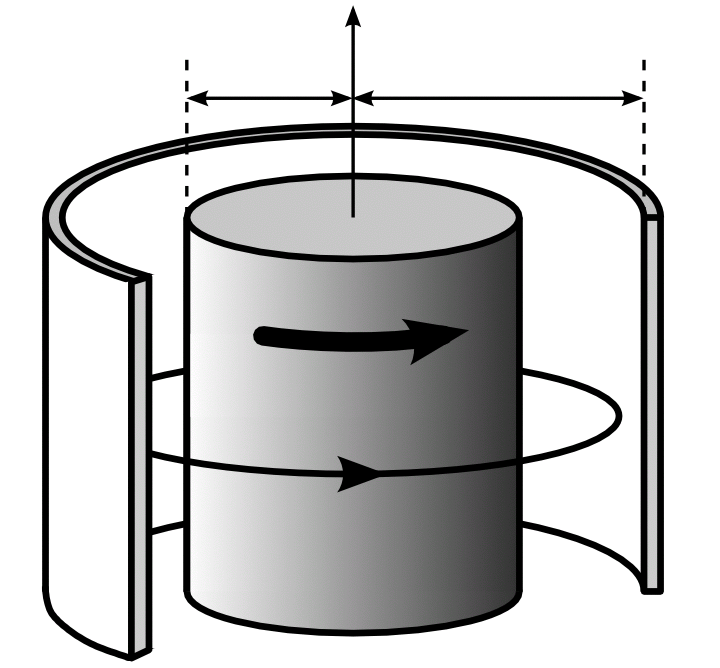
\includegraphics[width=40mm]{couette.pdf}}
		\put(35, 45){\vector(1, 0){7}}
		\put(43, 44){$U_1$}
		\put(2, 3.5){\vector(-1, 0){7}}
		\put(-10, 3){$U_2$}
		\put(8, 51){$y$}
		\put(30, 30){\color{bleu}$u(y) = 2by$}
	\end{picture}
\end{center}
\mycaption{Ecoulement de Couette entre deux plaques.}
\label{fig:couette}
\end{figure}


%%%%%%%%%%%%%%%%%%%%%%%%%%%%%%%%%%%%%%%%%%%%%%%%%%%%%%%%%%%%%%%%%%%%%%%%%%%%%%%%%%%%%%%%%%%%%%%%%%%
\end{document}
%%%%%%%%%%%%%%%%%%%%%%%%%%%%%%%%%%%%%%%%%%%%%%%%%%%%%%%%%%%%%%%%%%%%%%%%%%%%%%%%%%%%%%%%%%%%%%%%%%%

